\documentclass[journal]{IEEEtran}
\usepackage{cite}
% *** GRAPHICS RELATED PACKAGES ***
%
\ifCLASSINFOpdf
  \usepackage[pdftex]{graphicx}
\fi
%
\usepackage[cmex10]{amsmath}


% *** ALIGNMENT PACKAGES ***
%
\usepackage{array}
\usepackage{fixltx2e}

\usepackage{stfloats}
% LaTeX2e). It also provides a command:
\fnbelowfloat

\usepackage{booktabs}
\usepackage{amssymb}
\usepackage{amsmath}
\usepackage{pgf}
\usepackage{tikz}
\usetikzlibrary{arrows,positioning}
\usepackage{url}
\usepackage{color}
\usepackage{graphicx}
\usepackage{xspace}
\newcommand*{\eg}{e.g.\@\xspace}
\newcommand*{\ie}{i.e.\@\xspace}
\newcommand*{\vs}{vs.\@\xspace}

\newcommand*{\EMD}{\mathrm{EMD}}

% correct bad hyphenation here
\hyphenation{wave-let}

\usepackage{color}
\newcommand{\vl}[1]{\textcolor{orange}{Vincent : #1}}
\newcommand{\gl}[1]{\textcolor{red}{Gr\'egoire : #1}}
\newcommand{\ja}[1]{\textcolor{magenta}{Joakim : #1}}
\newcommand{\ml}[1]{\textcolor{blue}{ Mathieu : #1}}



\begin{document}
%
% paper title
% can use linebreaks \\ within to get better formatting as desired
% Do not put math or special symbols in the title.
%\title{An evaluation framework for event detection using a morphological model of acoustic scenes}
\title{Object-based Auditory Scenes Similarity Retrieval and Classification With Wavelet Scattering}

\author{Vincent Lostanlen\thanks{This work is supported by the ERC InvariantClass grant 320959.}, Gr\'egoire Lafay, Joakim And\'en, and Mathieu Lagrange}


% make the title area
\maketitle

% As a general rule, do not put math, special symbols or citations
% in the abstract or keywords.
\begin{abstract}

This paper introduces a generic hierarchical modeling scheme for acoustic scenes using the wavelet scattering transform at sub-second timescales with object-based segmentation at larger timescales. Application of the proposed approach to the acoustic scene similarity retrieval and acoustic scene classification tasks on publicly available datasets using a state-of-the-art classifier demonstrates the potential of featurs designed using the wavelet scattering transform, consistently outperforming baseline mel-frequency cepstral coefficients (MFCCs).

Also, representing the scene at larger time scale as a set of representative features of coherent segments is an effective approach for scene similarity retrieval as it allows the retrieval system to focus on discriminative features. 
\end{abstract}

% Note that keywords are not normally used for peerreview paper.
\begin{IEEEkeywords}
acoustic scene classification, acoustic scene segmentation, scattering, wavelets, earth mover's distance
\end{IEEEkeywords}

% For peer review papers, you can put extra information on the cover
% page as needed:
% \ifCLASSOPTIONpeerreview
% \begin{center} \bfseries EDICS Category: 3-BBND \end{center}
% \fi
%
% For peerreview papers, this IEEEtran command inserts a page break and
% creates the second title. It will be ignored for other modes.
\IEEEpeerreviewmaketitle

\section{Introduction}

\IEEEPARstart{T}{he} amount of audio data recorded from our sonic environment has grown considerably over the past decades.
In order to measure the effect of human activity and climate change on animal biodiversity, researchers in the field of ecoacoustics \cite{ECOACOUSTICS2014, krause} have recently undertaken the massive deployment of acoustic sensors throughout the world \cite{warren2006urban, NessSST13, stowell13a, stowell13b}. 

In addition, recent work demonstrates the interest of acoustic monitoring for the characterization of human pleasantness in urban areas \cite{lafayPartI, guyot2005urban, ricciardi2015sound} as well as the prediction of annoyance due to traffic \cite{gloaguen}.
Because they bear a strong societal impact and raise many scientific challenges, we believe that these case studies are of considerable interest for the signal processing community.

Formerly put, ecoacoustics is an interdisciplinary science that investigates natural and anthropogenic sounds and their relationship with the environment over a wide range of study scales at the intersection between ecology, acoustics and computer science. Despite identified needs, the field of signal-based ecoacoustics is still in infancy.
As a consequence, few well-built datasets are readily available for evaluation purposes.
A closely related, and more mature, field of investigation is the classification of acoustic scenes, where the aim is to predict labels by processing audio data. 

While narrower in its range of applications, it has the advantage of being rooted in cognitive psychology of categorization \cite{dubois2006cognitive, maffiolo_caracterisation_1999, guastavino_ideal_2006} and has received the attention of the data mining community for some time, resulting in the availability of several well-designed datasets.

Despite the differences, ecoacoustics and acoustic scene classification (ASC) task both raise the following question: how can we efficiently and effectively process a large amount of audio data using representations that are compact, generic in their design, and flexible in their use?

The work described in this paper attempts to answer this question by demonstrating the usefulness of two concepts: 1) using the wavelet scattering transform to extract discriminative features subject to a small number of parameters and 2) object-based modeling of the acoustic scene based on unsupervised clustering of each acoustic scene, allowing us to focus the scene description on specific areas of interest. \ja{Again, the last part is a little vague to me.}

Motivations of the proposed approach and a brief review of the state of the art in the field of acoustic scene modeling is given in Section \ref{sec:soa}. We describe the scattering transform in Section \ref{sec:scattering}, discuss post-processing transformations in Section \ref{sec:design} and propose a cluster-based scene description in Section \ref{sec:object}. In Section \ref{sec:experiments} several experiments are proposed for an unsupervised setting, \ie acoustic scene similarity retrieval (ASSR) and for a supervised setting, \ie acoustic scene classification (ASC). Results are subsequently reported in Section \ref{sec:results}.

\section{Background} \label{sec:soa}

%One avenue of ecoacoustics research, originating in bioacoustics, attempts to identify species properties of vocalizations, for example to link animal vocalization with behavior\cite{au2008principles, stowell2014large}.

A recent paradigm processes the audio stream in a holistic way over larger time scales, without assuming that a single species is present throughout the recording. Automated systems belonging to this paradigm aim to infer global properties of bioacoustic scenes, including biodiversity indices \cite{Bardeli2010}, migration patterns \cite{Obrist2010}, as well as to detect time regions of particular interest requesting detailed human inspection \cite{rosenstock2002landbird,diefenbach2007incorporating}.

%The same division is found in the field of auditory scene analysis, wherein the interest may either be 1) to isolate and identify precise events, \ie acoustic event detection (AED), or 2) to predict global attributes assigned to large time spans of audio, \ie acoustic scene classification (ASC).
In the latter, most state-of-the-art systems more or less follow the bag-of-frames (BOF) approach introduced by Acouturier et al. \cite{aucouturier2007bag}, where a scene is modeled by high-level summary statistics computed from local features.
Being a very generic method, this approach has been applied to many audio classification tasks besides ASC.
Yet the proposed implementation using Gaussian mixture models (GMMs) of mel-frequency cepstral coefficients (MFCCs) has been demonstrated comparably to a mere averaging of the features \cite{lagrange:hal-01082501}.
Indeed, the typical morphology of acoustic scenes is of a ``skeleton of events on a bed of textures'' \cite{nelken2013}, with a few discrete sound events superimposed upon a stationary acoustic background.
Therefore, it is arguably more beneficial to focus on the large-scale temporal evolution of auditory scenes rather on the joint probability distribution of short-term features.

This statement has some support in auditory psychology as well as sound synthesis based on summary statistics \cite{mcdermott2013summary}. Indeed, studies in cognitive psychology investigating urban sound environment quality pointed out that (perceived or measured) global sound level, are not sufficient to fully characterize an acoustic scene \cite{guyot2005urban,kang2006urban}. Rather, it seems that cognitive processes such as sound environment quality perception \cite{dubois2006cognitive} or loudness judgment \cite{kuwano_memory_2003} rely upon higher-level cognitive attributes such as the identities of sound sources which compose the scene. \ja{This argument is semantically a little tricky, since technically the low-level features already contain all this high-level information, it's just that the simple models we use to describe them fail to capture this high-level structure} It has been showed that, if available, the complete description of the scene in terms of event occurrences is powerful enough to reliably predict high-level cognitive classes, \textit{e.g.} the presence of birds are very likely to be heard in parks in urban areas and so are strong pleasantness indicators \cite{lafayPartI}. Consequently, research in sound perception is now strongly focused the contribution of specific sound sources in the assessment of a sound environment \cite{ricciardi2015sound,lavandier2006contribution}. Although the complete set of events occuring within a given auditory stream may not be discernable, even to human expects, research has shown that a small set of events, so-called markers, suffice to reliably predict many high-level attributes.

BOF approaches treats each observations equally, whereas the above cited results show that only a few events scarcely occurring may have be more important than events or texture present throughout the whole scene duration, thus advocating for a more selective approach such as the one presented in Section \ref{sec:object} for the ASSR task.

%\section{Background} \label{sec:soa}

Aside from \cite{aucouturier2007bag} and \cite{lagrange:hal-01082501} that consider the task of ASSR, much of the work dedicated to acoustic scene modeling is applied to the ASC tasks. \ja{Since we go into so much detail on ASC, shouldn't we at lest describe what these works do? Some of this is already described in the motivations section, so perhaps we should move some over in here?}
An overview of the efforts for the latter task is provided by the DCASE2013 challenge \cite{barchiesi2015acoustic}, held in 2013 to compare different approaches to scene classification. Table \ref{tab:dcase} summarizes the results of the submitted algorithms where most \ja{?} of scene predictions are achieved by majority voting of predictions over features. \ja{What about the other algorithms? Why are we excluding them here?}

\begin{table}
\begin{center}
\begin{tabular}{lcl}
& Acc. \%  &  \multicolumn{1}{c}{Design}  \\
\cite{olivetti2013wonder} OE & 17 & compression distance, random forests \\
\cite{elizalde2013vector} ELF & 55 & i-vector, LDA \\
\cite{krijnders2013tone} KH & 55 & cochleogram, SVMs \\
\cite{patil2013multiresolution} PE & 58 & 2D Gabor filters, SVMs \\
\cite{lee2013acoustic} NHL & 60 & UL of mel spectra, SVMs \\
\cite{nogueira2013sound} NR1 & 60 & MFCCs and ILD features, SVMs \\
\cite{chum2013ieee} CHR & 65 & sparsity features, HMMs  \\
\cite{geiger2013large} GSR & 69 & Mel-frequency Spectra and MFCCs, SVMs \\
\cite{rakotomamonjy2015histogram} RG & 69 & histogram of gradient (HOG), SVMs \\
\cite{li2013auditory} LTT & 72 & MFCCs, tree baggers \\
\cite{roma2013recurrence} RNH & 76 & RQA features stacked with MFCCs, SVMs \\
\end{tabular}
\end{center}
\caption{Designs submitted to the DCASE2013 ASC challenge. RQA stands for recurrence quantification analysis, ILD for inter-aural differences and UL for unsupervised learning. \label{tab:dcase}}
\end{table}

In this paper, we are interested in evaluating different algorithmic designs leading to different scene models, we therefore resort to straightforward ranking performance measures for the ASSR task. \ja{It's not clear to me how the first part implies the second part here} Similarly, we have picked SVMs as our classifier for the ASC task, since these are a standard tool in the community and allows for us to focus our analysis on the earlier processing stages. Moreover, since MFCCs are well-established features which perform well for these task, we shall include them baseline features in all experiments described in this paper.

%\gl{Othe this r paper:} \cite{jiang2005svm, kalinli2009saliency, su2011environmental, ye2015acoustic, bisot2015hog, chakrabarty2015exploring, xue2015auditory}

%\subsection{Datasets}

 % The latter is also considered in this paper as a validation of the proposed approach. \ja{What does this last sentence mean?}

%In this paper, we shall demonstrate that the use of features based on the wavelet scattering transform together with object-based representation of the acoustic scene allows us to achieve state-of-the-art \ja{?} performance in both the ASSR and ASC paradigms.

\section{Scattering representations \label{sec:scattering}}

Scattering transforms are time-shift invariant representations of audio signals consisting of auditory and modulation filter banks interspersed with complex modulus nonlinearities.
This section highlights the importance of invariance to time shifts and stability to time warps in the representation of acoustic scenes, and explains how the scattering transform is designed to satisfy these properties while having a high discriminative power.

\subsection{Invariance and stability in acoustic scenes}
The notion of invariance to time shifts plays an essential role in acoustic scene similarity retrieval as well as acoustic scene classification.
Indeed, recordings may be shifted locally without affecting their perception and therefore such shifts do not convey any information about the class.
To discard this superfluous source of variability, signals can be mapped to a time-shift invariant feature space before training the classifier, eliminating the need for the classifier to explicitly learn this invariance.
From any set of descriptors $\boldsymbol{x_1}(t,\gamma)$, where $\gamma$ denotes a descriptor index, a representation invariant to time shifts shorter in duration than $T$ can be obtained by convolving $\boldsymbol{x_1}$ with a low-pass filter $\boldsymbol{\phi}(t)$ of cutoff frequency set to $1/T$, as measured in Hertz:
\begin{equation}
\mathbf{S_1}\boldsymbol{x}(t, \gamma) = (\boldsymbol{x_1} \ast \boldsymbol{\phi}) (t).
\end{equation}
A downside is that the transient information in $\boldsymbol{x_1}$ at scales finer than $T$ are lost by this low-pass filtering, reducing discriminability in feature space.
To address this issue, the temporal scattering transform recovers this information by convolving $\boldsymbol{x_1}$ with wavelets whose center frequencies are above $1/T$ and then applying complex modulus.

By resorting to wavelet transform modulus, as opposed to Fourier transform modulus, the resulting features are provably stable to time-warping deformation,
in the sense of Lipschitz regularity with respect to diffeomorphisms \cite{Mallat2012}.
In addition to invariance, this stability property is crucial to signal classification, since it guarantees robustness to small variations in pitch, reverberation, and rhythmic organization of events, which make up an important part of the intra-class variability among natural sounds.

Starting from a monophonic waveform $\boldsymbol{x}(t)$, the scattering transform is defined as an infinite cascade of wavelet transform and modulus operators.
However, to achieve invariance to translation up to $T = 372\,\mathrm{ms}$, \ie the approximately minimal duration between non-overlapping acoustic events, two layers of scattering transform.

The next subsection describes the operations involved in temporal scattering, and in particular the construction of wavelet filter banks.

\ja{I'm not sure that this whole section makes sense right here. It can be a bit daunting to jump right in and talk about spectrograms $x_1$ and wavelets, etc. before we've defined them. Could we put this after the next subsection, explaining all the nice properties of the scattering transform and why we need them after we've defined it fully?}

\subsection{Temporal scattering}
Our convention for the Fourier transform of a continuous-time signal $\boldsymbol{x}(t)$ is $\boldsymbol{\hat{x}}(\omega) = \int x(t) \exp(\mathrm{i} 2\pi t \omega) \; \mathrm{d}\omega$. Note that the frequency variable $\omega$ is expressed in Hertz, not in radians per second.

Let $\boldsymbol{\psi}(t)$ a complex-valued band-pass filter of
center frequency $\xi_1$ and bandwidth $\xi_1/Q_1$.
A filter bank of wavelets is built by dilating $\boldsymbol{\psi}(t)$
according to a geometric sequence of scales $2^{\gamma_1/Q_1}$, obtaining
\begin{equation}
\boldsymbol{\psi_{\gamma_1}}(t) = 2^{-\gamma_1/Q_1} \boldsymbol{\psi}(2^{-\gamma_1/Q_1} t)\mbox{.}
\end{equation}
The variable $\gamma_1$ is the opposite number of a log-frequency, taking integer values between $0$ and $(J_1 \times Q_1 - 1)$.
In the sequel, we set $\xi_1$ to $20~\mathrm{kHz}$ (close to the Nyquist frequency of the audio recordings) the number of octaves $J_1$ to $10$ (the lower end of human hearing range) and the number of wavelets per octave $Q_1$ to $8$.
For each $\gamma_1$, the wavelet $\boldsymbol{\psi_{\gamma_1}}(t)$
has a center frequency of $2^{-\gamma_1/Q_1}\xi_1$, a bandwidth of $2^{-\gamma_1/Q_1}\xi_1/Q_1$, and a quality factor of $Q_1$.

The wavelet transform of an audio signal
$\boldsymbol{x}(t)$ is obtained by convolution with all wavelets.
Applying pointwise complex modulus the transform yields
the wavelet scalogram
\begin{equation}
\boldsymbol{x_1}(t, \gamma_1)
= \vert \boldsymbol{x} \ast \boldsymbol{\psi_{\gamma_1}} \vert (t)\mbox{.}
\end{equation}
The wavelet scalogram bears resemblance to the constant-Q transform (CQT),
which is derived from the short-term Fourier transform (STFT) by averaging the frequency
axis into constant-Q subbands of center frequencies $2^{-\gamma_1/Q_1}\xi_1$.
Indeed, both time-frequency representations are indexed by time $t$ and log-frequency $\gamma_1$.
However, contrary to the CQT, the wavelet scalogram reaches the Heisenberg
theoretical limit of optimal time-frequency localization across the whole
frequency range, whereas the temporal resolution of the CQT, at least in its original implementation \cite{Brown1992}, is fixed by the support of the STFT analyzing window.
Therefore, the wavelet scalogram has a better temporal localization at high
frequencies than the CQT, at the expense of a greater computational cost.
This increase in time-frequency localization comes at the expense of a greater computational cost, the inverse fast Fourier transform (IFFT) routine must be called for each wavelet $\boldsymbol{\psi_{\gamma_1}}$ in the filter bank.
Yet, it allows us to observe amplitude modulations at fine temporal scales in the scalogram, down to the minimum scale $2Q_1/\xi_1$ for $\gamma_1 = 0$, of the order of $1\,\textrm{ms}$ given the aforementioned values of $Q_1$ and $\xi_1$.

Among auditory scenes, amplitude modulations may be caused by a broad variety of mechanical interactions, including collision, friction, and turbulent flow.
At a longer scale, they also account for some higher-level attributes of sound, \eg prosody in speech or rhythm in music.
Although they are discarded while filtering $\boldsymbol{x_1}(t,\gamma_1)$ into a time-shift invariant representation $\mathbf{S_1}\boldsymbol{x}(t,\gamma_1)$, they can be recovered by a second wavelet transform modulus operator.
The amplitude modulation spectrum resulting from this operator is
\begin{equation}
\boldsymbol{x_2}(t,\gamma_1,\gamma_2) =
\vert \boldsymbol{x_1} \ast \boldsymbol{\psi_{\gamma_2}} \vert(t,\gamma_1),
\end{equation}
where the center frequencies of the wavelets $\boldsymbol{\psi_{\gamma_2}}(t)$ are of the form $2^{-\gamma_2/Q_2} \xi_2$, and the second-order log-frequency index $\gamma_2$ takes integer values between $0$ and $(J_2 \times Q_2 - 1)$. Note that these second-order wavelets are dilated versions of a second mother wavelet $\boldsymbol{\psi}$, with a different center frequency $\xi_2$ and quality factor $Q_2$. The identity of the wavelet will be clear from context.
In the sequel, we set $\xi_2$ to $2.5\,\mathrm{kHz}$, $Q_2$ to $1$, and $J_2$ to $12$. Lastly, the low-pass filter $\phi(t)$ is applied to $\boldsymbol{x_2}$ to guarantee invariance to time-shifting, which yields
\begin{equation}
\mathbf{S_2}\boldsymbol{x}(t,\gamma_1,\gamma_2) =
(\boldsymbol{x_2} \ast \phi)(t,\gamma_1,\gamma_2).
\end{equation}
The scattering transform consists of the concatenation of first-order coefficients $\mathbf{S_1}\boldsymbol{x}(t,\gamma_1)$ and second-order coefficients $\mathbf{S_1}\boldsymbol{x}(t,\gamma_1,\gamma_2)$ into a feature matrix $\mathbf{S}\boldsymbol{x}(t,\gamma)$, where $\gamma$ is a shorthand for either $\gamma_1$ or $(\gamma_1,\gamma_2)$.

\begin{figure}
\begin{center}
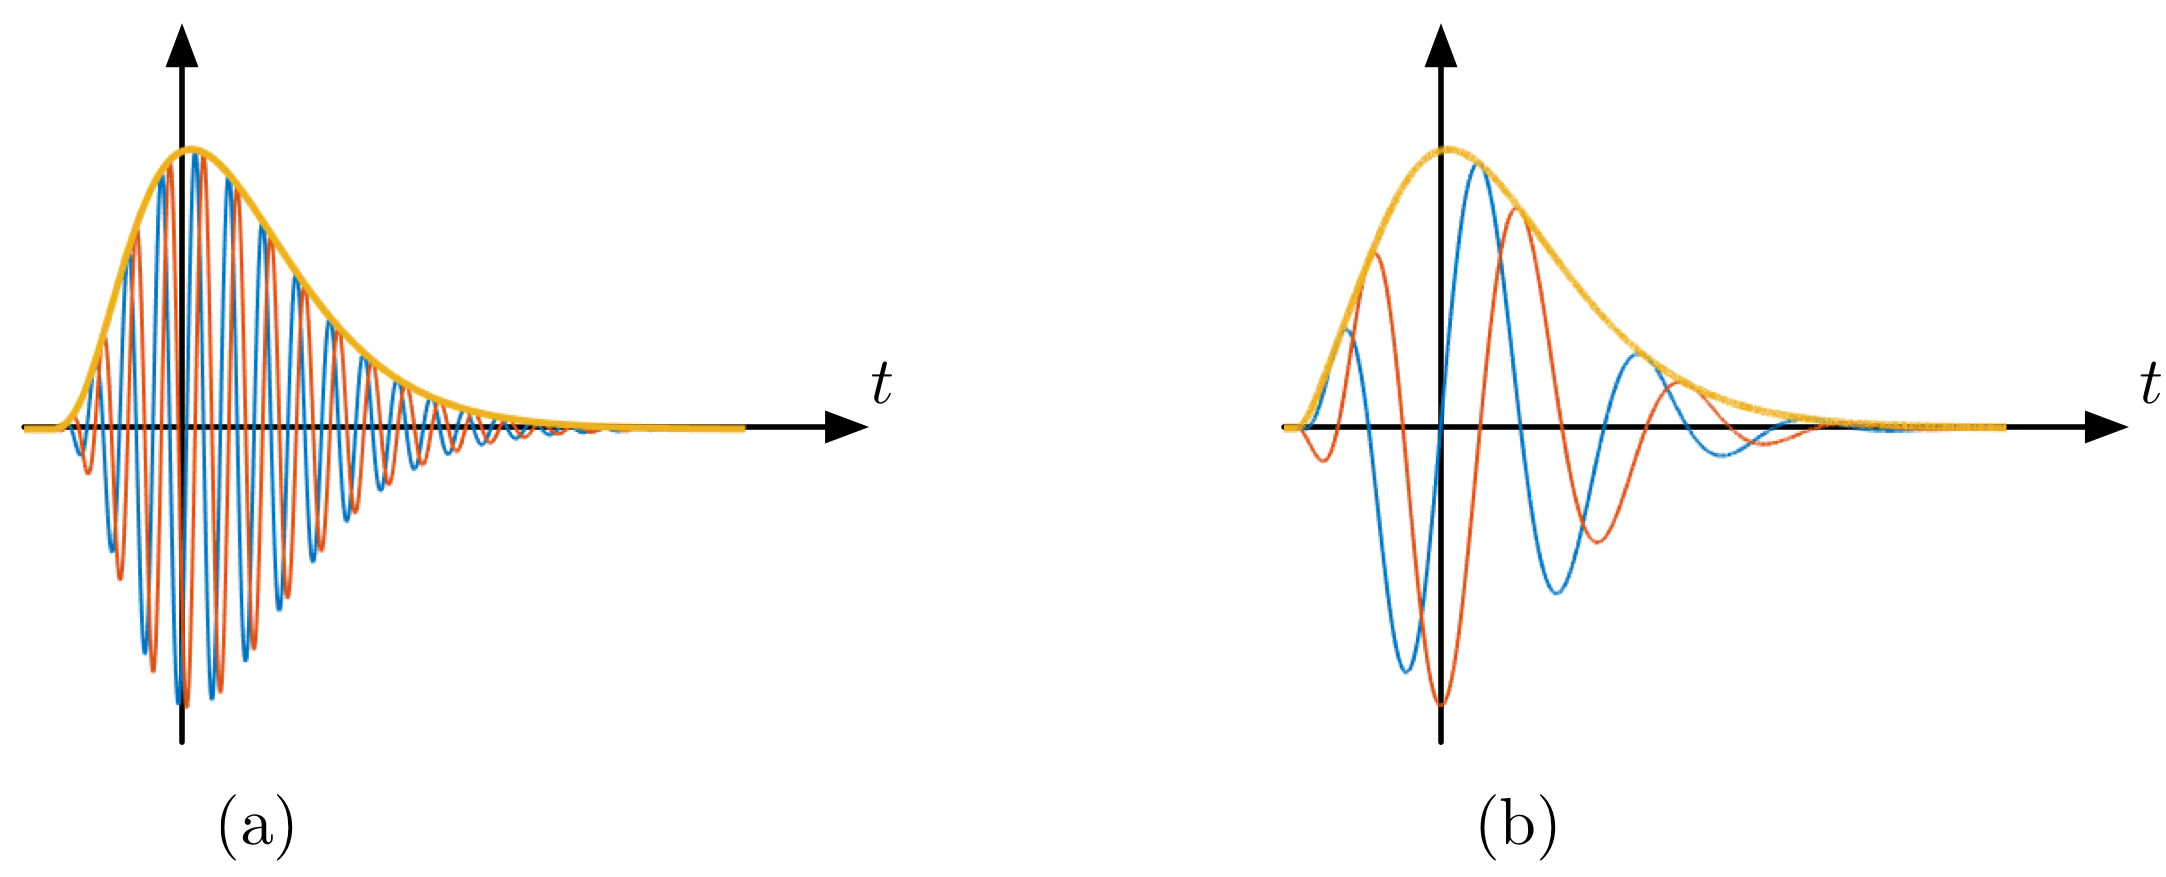
\includegraphics[width=\columnwidth]{gammatones.png}
\caption{
\label{fig:gammatones}
Gammatone wavelets $\psi(t)$ in the time domain with quality factors (a) $Q = 4$ and (b) $Q = 1$. Blue and red oscillations represent the real and imaginary parts. The orange envelope represents the complex modulus.}
\end{center}
\end{figure}

Wavelets
$\boldsymbol{\psi_{\gamma_1}}(t)$ and $\boldsymbol{\psi_{\gamma_2}}(t)$ are designed as fourth-order Gammatone
wavelets with one vanishing moment \cite{Venkitaraman2014}, as shown in Figure \ref{fig:gammatones}.
In the context of auditory scene analysis, the asymmetric envelope of Gammatone wavelets is more biologically plausible than the symmetric, Gaussian-like envelope of the more widely used Morlet wavelets.
Indeed, it allows to reproduce two important psychoacoustic effects in the mammalian cochlea: the asymmetry of temporal masking and the asymmetry of spectral masking  \cite{Fastl2007}.
Moreover, it should be noted that Gammatone wavelets follow the typical amplitude profile of natural sounds, beginning with a relatively sharp attack and ending with a slower decay. \ja{Why is this relevant for our classification task? Sparsity?}
As such, they can be discovered automatically by unsupervised encoding of natural sounds \cite{Smith2006}.

\section{Feature design}
\label{sec:design}
\ja{It seems that what we are doing in this section is more post-processing than feature design, which would be the scattering transform itself.}

Before supervised or unsupervised classification, it is beneficial to process scattering coefficients with feature transformations that improve invariance, normality, or generalization power.
In this section, we review three ways of achieving these properties, namely logarithmic compression, and temporal integration, and standardization.

\subsection{Logarithmic compression}
\label{sec:logcomp}

Many algorithms in pattern recognition, including nearest neighbor classifiers and support vector machines, tend to work best when all features follow a standard normal distribution across all training instances \cite{Hsu2003}.
Yet the distribution of the scattering coefficients is skewed towards larger values. We can reduce this skewness by applying a pointwise concave transformation, like a logarithm, to all coefficients.
Figure \ref{fig:histograms} shows the distribution of an arbitrarily chosen scattering coefficient over the DCASE2013 dataset, before and after logarithmic compression.

\begin{figure}
\begin{center}
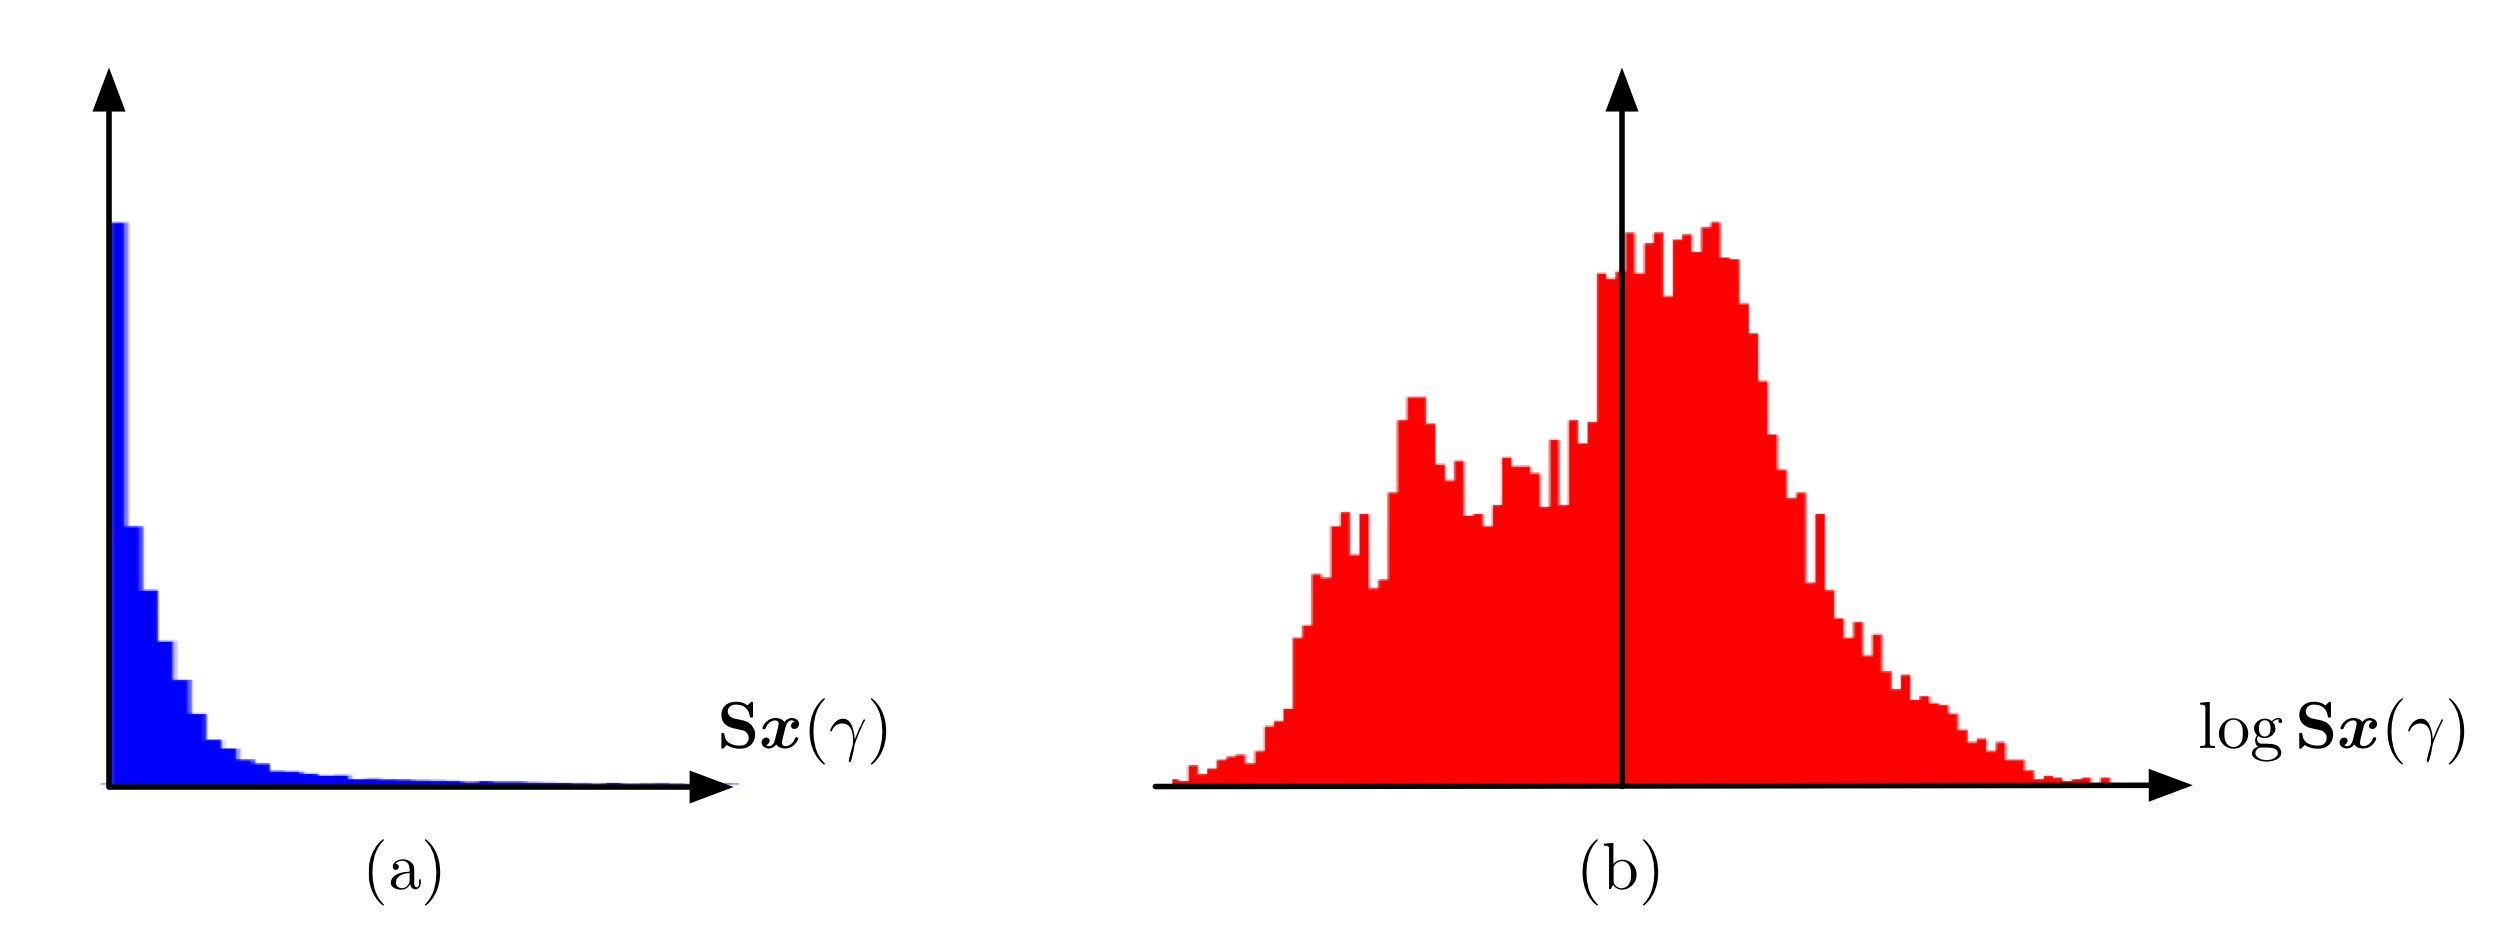
\includegraphics[width=\columnwidth]{compression.png}
\caption{
\label{fig:histograms}
Histogram of values taken by the first-order scattering coefficient $\mathbf{S}\boldsymbol{x}(\gamma)$, corresponding to a center acoustic frequency of $302\,\mathrm{Hz}$,
(a) before and (b) after logarithmic compression.}
\label{fig:compression}
\end{center}
\end{figure}


Taking the logarithm of a magnitude spectrum is ubiquitous in audio signal processing.
Indeed, it is corroborated by the Weber-Fechner law in psychoacoustics, which states that the sensation of loudness is roughly proportional to the logarithm of the acoustic pressure. 
We must also recall that the measured amplitude of sound sources often decays polynomially with the distance to the microphone, a source of spurious variability in scene classification.
Logarithmic compression can linearize this dependency, facilitating the construction of a powerful invariant at the classifier stage.

For the task of musical genre recognition, second-order scattering coefficients $\mathbf{S_2}\boldsymbol{x}(t,\gamma_1,\gamma_2)$ are sometimes normalized by the corresponding first-order scattering coefficients $\mathbf{S_1}\boldsymbol{x}(t,\gamma_1)$, since this decorrelates them from one another \cite{Anden2014}.
We note that taking the logarithm of such renormalized coefficients yields
\begin{equation}
\log \dfrac{\mathbf{S_2}\boldsymbol{x}(t,\gamma_1,\gamma_2)}{\mathbf{S_1}\boldsymbol{x}(t,\gamma_1)} =
\log \mathbf{S_2}\boldsymbol{x}(t, \gamma_1, \gamma_2) -
\log \mathbf{S_1}\boldsymbol{x}(t, \gamma_1),
\end{equation}
\ie a linear combination of the logarithms of first- and second-order coefficients.
As such, a non-linear renormalization becomes a linear transformation, which can be learned by a linearly discriminative classifier.

\subsection{Early \vs late temporal integration}
\label{sec:eili}

Owing to the scarcity of salient events in many natural scenes,
fine-grained classification is only made
possible by integrating signal information over a long temporal context.
Indeed, whereas a few seconds is often sufficient to recognize a speaker,
a musical instrument, or a genre, up to $30$ seconds may be required
to disambiguate two classes of auditory scenes with overlapping semantic content, \eg a train from a subway station or a quiet street from a park.
Depending on whether aggregation is performed in feature space or in decision space, the corresponding method is referred to as early or late integration.

A straightforward application of early integration consists in summarizing the multivariate time series of scattering coefficients over the full duration of the auditory scene, by retaining their average values only.
Going back to the definition of the scattering transform given in Section \ref{sec:scattering}, this is equivalent to increasing the support $T$ of the low-pass filter $\boldsymbol{\phi}(t)$ up to infinity. With a slight abuse of notation, we denote by
\begin{equation}
\mathbf{S}\boldsymbol{x}(\gamma) =
\int_{-\infty}^{+\infty} \mathbf{S}\boldsymbol{x}(t,\gamma)\;\mathrm{d}t
\end{equation}
the summarized features.

Conversely, a late integration scheme relies on probabilistic assignments $\mathbb{P}\left[y \,\vert\, \mathbf{S}\boldsymbol{x}(t,\gamma) \right]$ over short-term windows of length $T$, which are subsequently aggregated to produce a final decision
\begin{equation}
\hat{y} = \arg \max_{y} \rho\Big(\big\{ \mathbb{P}\left[y \,\vert\, \mathbf{S}\boldsymbol{x}(t,\gamma) \right] \big\}_{t} \Big)\mbox{,}
\end{equation}
where $\hat{y}$ is the estimated class label and $\rho$ is a reduction function, such as sum, product, or majority vote \cite{Kittler1998}.

A drawback of early integration is that it drastically reduces the number of training instances at the classifier stage, down to one per auditory scene.
In the context of the DCASE 2013 dataset, this corresponds to merely $8$ training instances per class, and $80$ instances overall, hence an increase in variance in statistical estimation and a risk of overfitting. \ja{That may be, but by averaging, we also reduce the variability of our data, which may be a good thing. If we're dealing with Gaussian processes, this is in fact a very good thing to do.}
On the contrary, a late integration scheme for $T=372\textrm{ ms}$ would yield $128$ instances per auditory scene \ja{How long is each recording? Should we specify this somewhere?}, resulting in $10240$ instances overall.
However, many of these instances may be silent or lack any salient properties of the class they are assigned to, hence an increase in bias and a risk of underfitting.
In short, early and late integration methods lie at opposite ends of the bias-versus-variance statistical tradeoff. We refer to \cite{Joder2009} for a comprehensive review of this problematic in the context of musical instrument recognition. \ja{Another important difference is that early integration makes the classifier objective more appropriate, since the SVM will maximize the final classification error on the training data, as opposed to some intermediate frame-level label.}
In the context of this paper, early integration refers to an averaging of the features and late integration refers to a majority voting of the predictions. 
%\ja{We should perhaps mention this in that particular section instead of over here.}
\subsection{Standardization}
\label{sec:stand}

Let $\mathbf{S}\boldsymbol{X}(\gamma,n)$ be a dataset, where the indices $\gamma$ and $n$ respectively denotes features and examples.
It is commonly acknowledged that SVMs should be trained on scaled features with null mean and unit variance, so as to avoid mismatch in numeric ranges. \ja{Again, it would be really good if we could cite something for this.}
This operation may also help making the dataset linearly separable in feature space. \ja{Why?}
To standardize $\mathbf{S}\boldsymbol{X}(\gamma,n)$, we apply the affine transformation
\begin{equation}
\widetilde{\mathbf{S}}\boldsymbol{X}(\gamma, n) =
\dfrac{ \mathbf{S}\boldsymbol{X}(\gamma, n) -
\mu[ \mathbf{S}\boldsymbol{X}](\gamma)}{\sigma[ \mathbf{S}\boldsymbol{X}](\gamma)}
\end{equation}
where $\mu[ \mathbf{S}\boldsymbol{X}](\gamma) = \frac{1}{N} \sum_{n=1}^{N} \mathbf{S}\boldsymbol{X}(\gamma,n)$ is the sample mean of $\mathbf{S}\boldsymbol{X}(\gamma,n)$ and
\begin{equation}
\sigma[\mathbf{S}\boldsymbol{X}] (\gamma) =
\sqrt{\frac{1}{N-1} \sum_{n=1}^{N}
\left( \mathbf{S}\boldsymbol{X}(\gamma,n) - \mu[\mathbf{S}\boldsymbol{X}] \right)^2}
\end{equation}
is the sample standard deviation.

The vectors $\mu[\mathbf{S}\boldsymbol{X}(\gamma)]$ and $\sigma[\mathbf{S}\boldsymbol{X}](\gamma)$ are estimated from the training set only, and the same affine transformation is subsequently applied to all samples in the training set and the test set.

\section{Object-based modeling of the scene}
\label{sec:object}

%As part of the aforementioned research areas and applications, the emerging field of \emph{Acoustic Scene Analysis} (also called \emph{Sound Scene Analysis}) \cite{Stowell15} aims to develop approaches and systems for the automatic analysis of environmental sounds and soundscapes (originating both from urban or nature environments). While research methodologies in related fields such as Automatic Speech Recognition (ASR) \cite{Rabiner93} and Music Information Retrieval (MIR) \cite{Muller07} are now well established, research addressing Acoustic Scene Analysis remains relatively young. 

%From a data processing point of view, a holistic scheme, such as the bag-of-frame approach \cite{aucouturier2007bag}, has a simplicity, but clearly face poor performance on realistic conditions \cite{lagrange:hal-01082501}. 

As discussed in Section \ref{sec:motivations}, results in sound perception suggest the appropriateness of an object-based representation of auditory scenes for predicting high-level properties. That being said, perfect knowledge of which event occurred at a given time is not feasible. \ja{What does this mean?} In this paper, we therefore focus on a simple quantization scheme that is as generic as possible, implemented using a clustering approach where coherent regions of the scene are identified. The clustering is done using the centroid-based clustering algorithm KMeans.

Given a set a $d$-dimensional feature vectors $x_l^u\in X_u$, $l=[1,2,\ldots,L]$, extracted from the scene $s_u$, $u=[1,2,\ldots,U]$, the goal of KMeans is to partition $X_u$ into $M$ clusters $c^u_m\in C_u$, $m=[1,2,\ldots,M]$. The partitioning is done by minimizing for each $m$ cluster the squared error between its empirical mean (centroid) and the points it contains. Given $\mu_m^u$ the centroid of the cluster $c_m^u$, KMeans minimizes the following objective function:

\begin{equation}
J(C_u)=\sum\limits_{m} \sum_{x^u_l\in c^u_m} \vert \vert x_l^u - \mu_m^u \vert \vert^2
\end{equation}

At the end, each scene $s_u$ is described by a set of clusters $C_u$. One should note that this quantization approach differs from unsupervised learning schemes such as the ones studied in \cite{bisot2016acoustic}, where the scene features are projected in a dictionary learned from the entire dataset.

%which clusters not over a single scene, but over the whole dataset, and re-projects each scene in the resulting enhanced feature space. \ja{This sentence is also a big unclear.}

Here, with the aim of better balancing the influence of salient sound events and texture-like sounds on the final decision, the similarity between two scenes is computed based on their centroids similarities.

The similarity between all the scene centroids $\mu_i$, $i=[1,2,\ldots,I]$ with $I=UM$, is computed using a radial basis function (RBF) kernel $K$ combined with the local scaling method proposed in \cite{selfTuneManor2004}:
\begin{equation}
\label{eq:kc}
K_{ij} = \exp\left( - \dfrac{\Vert \mu_i - \mu_j \Vert^2}{\Vert \mu_i - \mu_{k,i} \Vert \Vert \mu_j - \mu_{k,j} \Vert} \right) 
\end{equation} 

where $\mu_{k,i}$ and $\mu_{k,j}$ are the $k^{\textrm{th}}$ nearest neighbor to the centroids $\mu_i$ and $\mu_j$ respectively, and $\Vert \cdot \Vert$ denotes the Euclidean norm.

To compute the similarity between two scenes, we then consider several centroid-based similarity metrics:

\begin{itemize}
\item \emph{ob-closest} (ob-c): the similarity between two scenes is equal to the largest similarity between their centroids,
\item \emph{ob-averaged} (ob-a): the similarity between two scenes is equal to the average of their centroids similarities, and
\item \emph{ob-weighted} (ob-w): for each scene, each centroid is weighted according to the number of frames belonging to its cluster. Each scene $s_u$ is thus described by a signature $p_u$ of $M$ clusters ($p_u=\lbrace(\mu_1^u,w_1^u),(\mu_2^u,w_2^u),\ldots,(\mu_M^u,w_M^u)\rbrace$), with $\mu_m^u$ and $w_m^u$ being the centroid and the weight of the $m$th cluster respectively. A cross-bin histogram distance, taking into account both the clusters weights of the scenes and the distances between their cluster centroids is then used. 
\end{itemize}

For \emph{ob-w}, the cross-bin histogram distance used is a variant of the earth mover's distance ($\EMD$), known as $\widehat{\EMD}$ and introduced in \cite{pele2008linear}. $\EMD$ computes the distance between two histograms by finding the minimal cost to be paid to transform one histogram into the other. An advantage of $\EMD$ is that it automatically aligns the histogram bins by using a ``ground distance'' which is the distance between the bin centers in the two histograms. In our case, the histograms are the clusters weights $w^u$ defined over the bins formed by clusters centroids $\mu^u$.

The $\widehat{\EMD}$ variant of $\EMD$ is adapted for non-normalized histograms. To compute the $\widehat{\EMD}$, we use the implementation proposed in \cite{pele2009fast}. Given two signatures $p_u$ and $p_v$ made of $n$ and $m$ clusters respectively, the $\widehat{EMD}$ is computed by solving the following linear programming problem:

\begin{equation}
\begin{split}
\widehat{\EMD}(p_u,p_v) &=\left( \min\limits_{\lbrace f_{nm}\rbrace} \sum\limits_{n,m} f_{nm}D_{nm}^{uv} \right) \\
&+ \left|\sum\limits_{n} w_n^u - \sum\limits_{m} w_m^v  \right| \alpha \max\limits_{n,m}\lbrace  D_{nm}^{uv}\rbrace
\end{split}
\end{equation}

\begin{equation*}
\mathrm{s.t.} \quad f_{nm}\geq0 \quad \sum\limits_{m} f_{nm} \leq w_n^u \quad \sum\limits_{n} f_{nm} \leq w_m^v
\end{equation*}

\begin{equation*}
\sum\limits_{n,m}f_{nm} = \min\left( \sum\limits_{n} w_n^u ,\sum\limits_{m} w_m^v \right)
\end{equation*} \ja{Can we provide some interpretation for the different terms and constraints here?}
where $\lbrace f_{nm} \rbrace$ is the flow between the cluster weights $w_n^u$ and $w_m^v$, that is, the amount transported from the $n$th bin to ``supply the demand'' of the $m$th bin. We denote by $D^{uv}$ the ground distance, a matrix containing the pairwise distances between the centroids sets $\mu^u$ and $\mu^v$. $D^{uv}$ is computed from the kernel $K$:
\begin{equation*}
D^{uv}=1-K^{(uv)}
\end{equation*}
with $K^{(uv)}$ being the slice of $K$ containing the pairwise similarities between the centroids sets $\mu^u$ and $\mu^v$ of the scenes $s_u$ and $s_v$ respectively. As suggested in \cite{pele2009fast}, we set the tradeoff parameter $\alpha$ to $1$.

To get the final similarity measure between the scenes $s_u$ and $s_v$, an extended Gaussian kernels $K^s$ \cite{chapelle1999support,jing2003support} is computed:
\begin{equation}
\label{eq:ks}
K_{uv}^s = \exp\left( - \dfrac{\widehat{\EMD}(p_u,p_v)}{A} \right) \\
\end{equation}
with $A$ a scaling parameter, set to the mean value of the $\widehat{\EMD}$ between all the scenes. The resulting kernel $K^s$ is known as an EMD kernel, and it should be noted that there is no guarantee that this kernel is positive definite.

\section{Experiments}
\label{sec:experiments}

\subsection{Datasets}

%For most of the experiments reported in this paper, we will consider the DCASE2013 dataset \cite{giannoulis2013database, 7100934}. Larger datasets exists: the
%Rouen dataset \cite{rakotomamonjy2015histogram} and the public part of the DCASE2016 challenge.%

In the experiments reported in this paper, the DCASE2013 \cite{giannoulis2013database, 7100934} and the public part of the DCASE2016 datasets  \cite{Mesaros2016_EUSIPCO} are considered. To build the DCASE2013 dataset, three different recordists visited a wide variety of locations in Greater London over
a period of several months and in each
scene recorded a few minutes of audio. No
systematic variations in the recordings covaried with scene
type: all recordings were made under moderate weather conditions, at varying times of day and week, and each recordist recorded each scene type.
The dataset is split into a public dataset that can used for optimizing the ASC system and a private dataset used for computing the resulting accuracy using a fivefold cross validation scheme. The folds used in this paper are the same as the ones used during the challenge. 

The DCASE2013 dataset has significant intra-class diversity while remaining manageable in terms of size, making it suitable for extensive evaluation of algorithmic design choices \cite{lagrange:hal-01082501}. In addition, it is still challenging, with a state-of-the-art system based on feature design \ja{?} and SVMs achieving $76\%$ \cite{roma2013} (winner of the DCASE2013 challenge). Another system, using a HOG+SVM approach \cite{rakotomamonjy2015histogram}, achieves $75\%$ and $92\%$ on the DCASE2013 and Rouen datasets, respectively. Recent advances using hierarchical classifier architectures obtain between $84\%$ and $87\%$ on DCASE2013 depending on the prior knowledge used during training \cite{phan2016label}. On the Rouen dataset, the state-of-the-art is currently $95\%$ \cite{bisot2016acoustic}.


\subsection{Feature design}

Experiments are carried out using temporal scattering coefficients as well as mel-frequency cepstral coefficients (MFCCs) as features. For the temporal scattering, each scene is described by $128$ vectors of scattering coefficients computed with half-overlapping windows $\boldsymbol{\phi}(t)$ of duration $T=372\,\mathrm{ms}$. Experiments are conducted with and without the logarithmic compression (see Section \ref{sec:logcomp}).

Different sets of parameters were tested to compute the MFCCs. Results here are only reported for the best setting, which consisted of $40$ MFCCs (including the first energy coefficient) computed for windows of $50\,\mathrm{ms}$ and hops of $25\,\mathrm{ms}$, with full frequency range. This setting gives us $600$ feature vectors per scene. To get a more robust representation of lower dimensionality a pooling step is performed on the MFCCs: each recording is divided into $n$ non-overlapping $t$-seconds long ``texture'' windows. The MFCC vectors within each texture window are then averaged in time. As the \emph{ob} approaches involve a clustering step, we need to ensure that both MFCCs and scattering coefficients have a comparable number of vectors per recording. \ja{Why do we need to do this?} Thus, $t$ is set to $250\,\mathrm{ms}$, resulting in $120$ MFCCs texture windows per scene.

\ja{We've tested the impact of the logarithm here, but not of the feature selection or standardization. Should we do this as well? For the feature selection, we did say earlier that we would test its impact.}

\subsection{Methods}

The influence of the temporal scattering transform and the \emph{ob} approaches are assessed in an unsupervised setting (ASSR) and in a supervised setting (ASC).

For ASSR, evaluation is performed on the private part of the DCASE2013 dataset. The metric used is the precision at rank $k$ ($p@k$), which is computed by taking a query item and counting the number of items of the same class within the $k$ closest neighbors, and then averaging over all query items. The $p@k$ is computed for $k=\{1,\ldots,9\}$, since each class only has $10$ items \ja{?}. Note that a $p@1$ is equivalent to the classification accuracy obtained by choosing the label of the closest neighbor for a given item. For each experimental setting, we only report the results obtained with the sets of parameters, \emph{i.e.} the number of clusters $m$ for the \emph{ob} approaches and the scaling parameter $N$ of the RBF kernels (see Eq. \ref{eq:kc}) leading to the best $p@9$. \ja{I'm not sure what this means. Do we fix $m$ and $N$ here for all experiments or do we optimize them over the test data each time? If so, this will bias the results, no?}
 
For ASC, the systems are again evaluated on the private part of DCASE2013, but here with five-fold stratified cross validation. The folds are identical to those used in the original challenge. Optimal parameters (see above) are this time learned on the public part of the DCASE2013 dataset, also using five-fold stratified cross validation. Clustering is done using KMeans$++$ \cite{arthur2007k}, an augmented version of K-means with a robust initialization procedure.

The \emph{ob} approaches are compared to commonly used early integration approach (\emph{early}) for ASSR, while both early and late integration (\emph{late}) strategy are evaluated for the ASC setting (see Section \ref{sec:eili}).

In the same way as the majority of the DCASE2013 participants, we use an SVM for the ASC task, which is a large-margin binary discriminator with tunable regularization of misclassified examples. The parameter $C$ is here set to $1$.

For the \emph{ob} approaches, we use the precomputed kernels described in Section \ref{sec:object}. For both the \emph{early} and \emph{late} approaches, a linear kernel as well as a RBF kernel are used. As in the RBF kernels used in the \emph{ob} approaches, the RBF kernel in the SVM is scaled locally using the method proposed in \cite{selfTuneManor2004}. All feature vectors, be they frames, texture windows or centroids, are standardized prior to be given to the classifier. The standardization is computed with respect to the train/test splits of the cross validation scheme (see Section \ref{sec:stand}).

\section{Results \label{sec:results}}

\begin{figure}
\begin{center}
\includegraphics[width=8cm]{gfx/unsupervised_test3.eps}
\caption{ASSR: $p@k$ obtained for MFCCs and scattering with logarithmic compression.}
\label{fig:ASS_1}
\end{center}
\end{figure}

\begin{figure}
\begin{center}
\includegraphics[width=8cm]{gfx/unsupervised_test2.eps}
\caption{ASSR: $p@k$ obtained for scattering with and without logarithmic compression.}
\label{fig:ASS_2}
\end{center}
\end{figure}

\subsection{Acoustic Scene Similarity Retrieval}

This section presents evaluation results for the ASSR settings. The $p@k$ for different settings are shown in Figures \ref{fig:ASS_1} and \ref{fig:ASS_2}, illustrating the effect of the different similarity metrics and the influence of the logarithm, respectively.

\subsubsection*{MFCC \vs scattering transform}

Irrespective of the rank $k$ considered, best result is achieved for the scattering transform with logarithmic compression using the \emph{ob-c} approach. Overall, log-compressed scattering coefficients systematically outperform MFCCs. This is to be expected since the scattering coefficients capture larger-scale modulations as opposed to the MFCCs which only describe the short-time spectral envelope.

\subsubsection*{Object-based \vs early integration}

For the scattering transform, \emph{ob-c} and \emph{ob-w} outperform \emph{early}, thus confirming the benefits of using an object-based representation to refine the similarity measures between the scenes. However, it is worth noticing that \emph{ob-a} perform equivalently to \emph{early}, which shows that the discriminant information is destroyed by averaging the contributions from all centroids. To take advantage of an object-based representation, we need to select certain representative centroids when comparing objects. Furthermore, it appears that \emph{ob-c} is be able to better characterize the classes than \emph{ob-w}. This last observation suggests that weighting a centroid according to the number of frames it contains may prove to be a limited solution. Indeed, nothing a priori indicates that the discriminant information between two scenes lays within the majority of their frames. On the contrary, two similar environments may shared a lot of similar sound sources with only a few sources discriminating between them.

For the MFCCs, there is no clear evidence that the \emph{ob} approaches improve the results. \ja{Why?}

\subsubsection*{Role of logarithmic compression}

Outcomes for the scattering with and without logarithmic compression are shown in Figure \ref{fig:ASS_2}. It can be seen that the logarithmic compression strongly improves the results, especially for the \emph{ob} approaches, which perform worse than \emph{early} without the logarithmic compression. \gl{une idée du pourquoi ?}

\subsection{Acoustic Scene Classification}
We report experiments on acoustic scene classification (ASC), following the original methodology of the DCASE 2013 challenge, and extend our approach to the its 2016 edition.

\subsubsection*{MFCCs \vs scattering}
as shown in Figure \cite{folds}, scattering coefficients outperform MFCCs over all but one fold of the DCASE 2013 private dataset when applying early integration, and over all folds when applying late integration.
Not only the average accuracy is improved, but the variance between fold-wise accuracies is also reduced, \eg from $16\%$ to $7\%$ in the case of early integration.
This is in accordance with the previous results on similarity retrieval, as well as with other papers comparing mel-frequency coefficients with scattering coefficients on a variety of tasks, ranging from musical genre recognition \cite{Anden2014} to environmental sound classification \cite{Salamon2015}.

\subsubsection*{Early \vs late integration}
late integration, \ie building a prediction by majority voting over $128$ local windows of duration $T=372\,\mathrm{ms}$, outperforms early integration, \ie classifying the acoustic scene with a global window of duration $T=24\,\mathrm{s}$.
This result suggests that, despite its discriminative power at fine scales, the scattering transform is unable to segregate distinct acoustic events beyond the scale of about one second.
Therefore, it is beneficial to regard the scattering transform as a mid-level descriptor of acoustic content, not as a high-level descriptor, and adopt a data-driven strategy for the temporal integration of acoustic events within one scene.
Surprisingly, although we ran an extensive number of experiments to formulate object-based clustering into a supervised setting for acoustic scene classification, none of them managed to outperform the baseline strategy in temporal integration, namely majority voting.

\subsubsection*{Role of logarithmic compression}
logarithmic compression provides a small, albeit consistent boost to acoustic scene classification over all folds in the DCASE 2013 private dataset.
Indeed, as discussed in subsection \ref{sec:logcomp}, and observed in Figure \ref{fig:compression}, the statistical assumption of normality for scattering coefficients is only approximately satisfied once mapped to a logarithmic, decibel-like scale.
This transformation improves the discriminative power of support vector machines (SVM) trained on scattering coefficients, whatever be the chosen temporal integration strategy (early or late) or the inner product kernel (linear or Gaussian RBF).
Again, this is in accordance with our previous findings on acoustic scene similarity retrieval, which are reported in Figure \ref{fig:ASS_2}.

\begin{figure}
\begin{center}
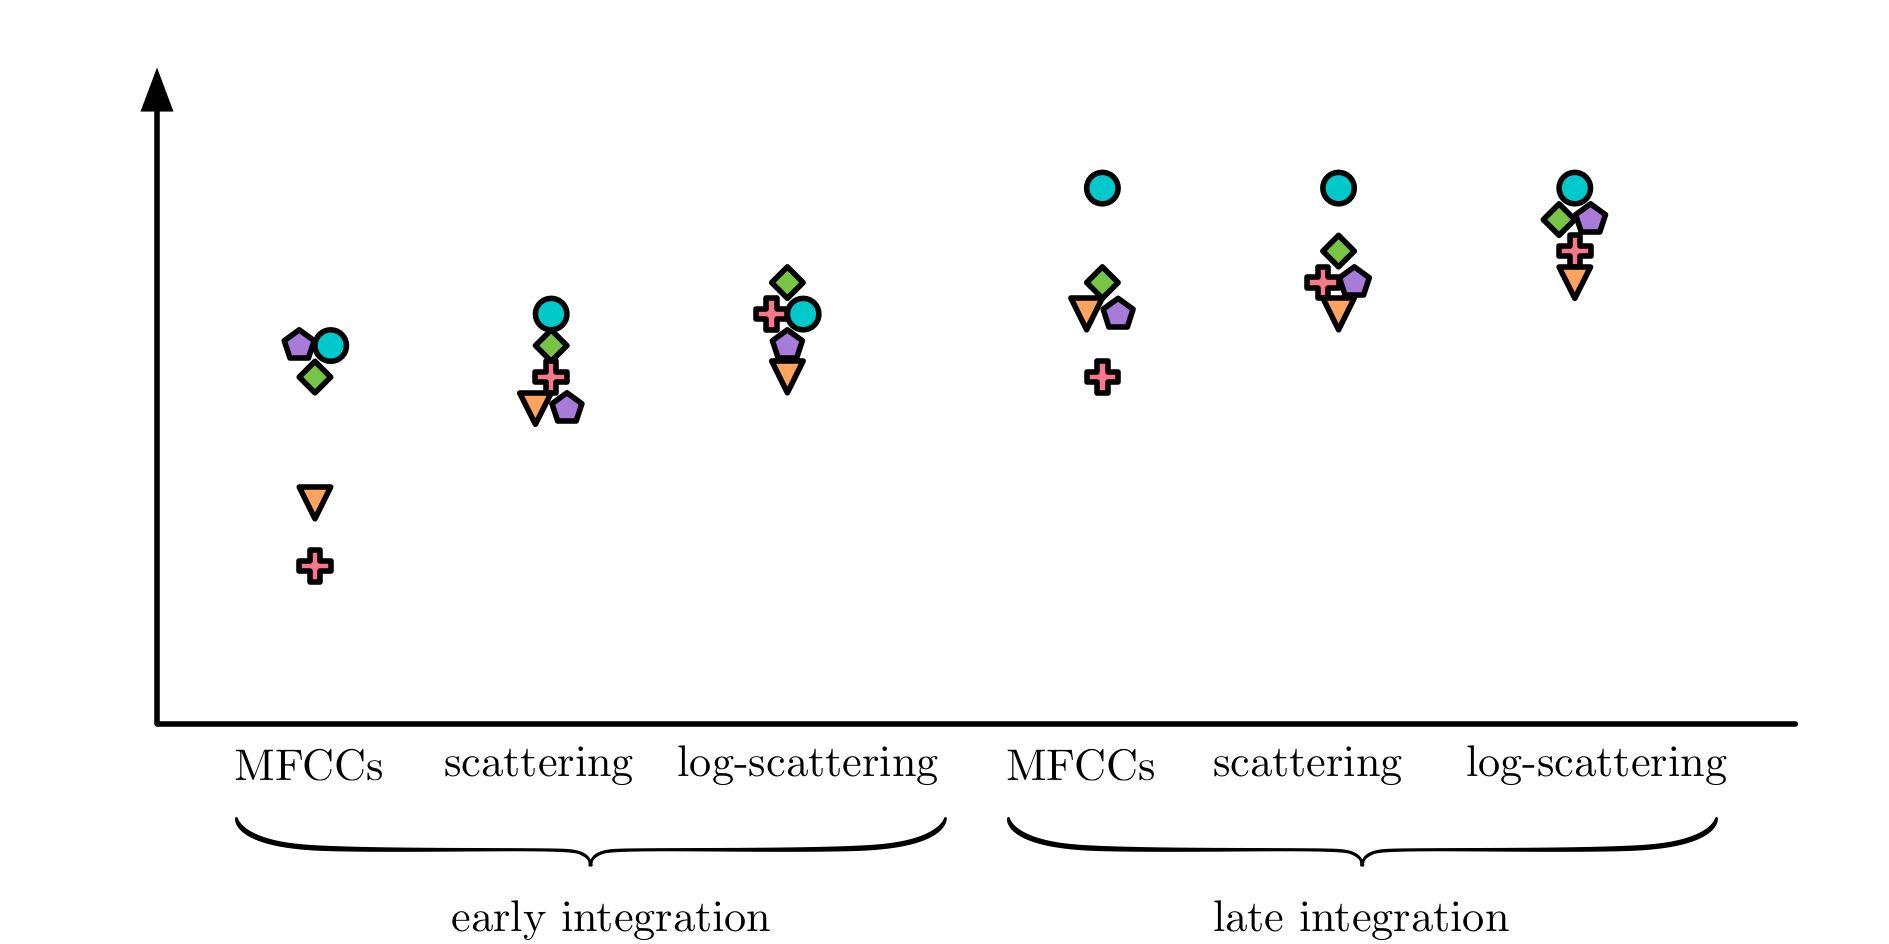
\includegraphics[width=\columnwidth]{folds.png}
\caption{Classification accuracies over the five folds of the DCASE 2013 private dataset, for various acoustic descriptors and temporal integration strategies. 
The chosen classifier is a support vector machine (SVM) whose kernel is a Gaussian radial basis function (RBF).
The mean accuracies and fold-wise standard deviations of each experiment are reported in Table \ref{table:dcase2013}}
\end{center}
\label{fig:folds}
\end{figure}


\begin{table}
\begin{center}
\begin{tabular}{llll}
             & MFCCs         & scattering & log-scattering  \\
             \hline
early, linear  & $54\pm20$   & $62\pm\phantom{0}6$  & $66\pm11$     \\
early, RBF     & $47\pm16$  & $56\pm\phantom{0}7$  & $63\pm\phantom{0}6$   \\
late, linear  & $60\pm\phantom{0}9$ & $70\pm\phantom{0}8$  & $75\pm\phantom{0}5$   \\
late, RBF     & $68\pm10$ & $73\pm\phantom{0}8$  & $\mathbf{78}\pm\phantom{0}6$   \\
\end{tabular}
\caption{Classification accuracies on the DCASE 2013 dataset with various settings of features, temporal integration strategies, and support vector machine kernels.}
\end{center}
\label{table:dcase2013}
\end{table}

\subsubsection*{Participation to the DCASE 2016 challenge}
In order to evaluate how general our findings are, we have taken part in the acoustic scene classification task 2016 edition of the DCASE challenge, whose results are forthcoming.
This edition relies on the TUT 2016 acoustic scenes dataset, which contains $15$ classes of acoustic scenes, and is larger than the DCASE 2013 private dataset by one order of magnitude \cite{Mesaros2016_EUSIPCO}.
Training support vector machines with a Gaussian RBF kernel is computationally demanding for a dataset of such size, especially under a late integration scheme, wherein the number of training instances exceeds $10^5$.
Since the LIBLINEAR package enables faster training than LIBSVM, we have used a linear kernel \cite{Hsu2003}.
Our experiments on the DCASE 2013 dataset, as reported in table \ref{table:dcase2013}, show that the linear kernel gives comparable, albeit slightly worse, classification results than the Gaussian RBF kernel.

Our results on the development dataset are reported in Table \ref{table:dcase2016}, in comparison with a baseline of $MFCCs$ coefficients and a generative classifier, namely Gaussian mixture models with $16$ Gaussians per model.
The average accuracy across classes is brought from $70.8\%$ to $79.4\%$.
The results on the evaluation dataset are awaiting publication by the DCASE organizing committee, and will be disclosed in August 2016.


\begin{table}
\begin{center}
\begin{tabular}{lcc}
Features & MFCCs & log-scattering \\
Classifier  & GMMs    & linear SVMs \\
Temporal integration & late (product rule) & late (majority voting) \\
\midrule
beach & $74.6 \pm 18.9$ & $83.5 \pm \phantom{0}7.1$ \\
bus & $58.2 \pm 18.3$ & $88.8 \pm 11.4$ \\
caf\'{e} / restaurant & $85.1 \pm 10.8$ & $64.5 \pm \phantom{0}8.3$ \\
car & $69.1 \pm 20.8$ & $94.9 \pm \phantom{0}6.1$ \\
city center & $89.6 \pm \phantom{0}9.2$ & $91.7 \pm \phantom{0}9.4$ \\
forest path & $72.4 \pm 23.8$ & $93.8 \pm \phantom{0}7.8$ \\
grocery store & $74.1 \pm 13.7$ & $90.9 \pm \phantom{0}6.9$ \\
home & $78.1 \pm 17.7$ & $56.2 \pm 23.9$ \\
library & $65.1 \pm 23.3$ & $82.0 \pm 13.0$ \\
metro station & $85.2 \pm 15.6$ & $96.0 \pm \phantom{0}2.3$ \\
office & $90.8 \pm 16.0$ & $87.5 \pm 21.7$ \\
park & $25.6 \pm 11.0$ & $75.4 \pm \phantom{0}7.4$ \\
residential area & $75.1 \pm 19.4$ & $44.2 \pm 15.0$ \\
train & $34.1 \pm \phantom{0}7.2$ & $58.3 \pm 10.0$ \\
tram & $85.4 \pm 13.9$ & $83.7 \pm 12.2$ \\
\bottomrule
Average & $70.8 \pm \phantom{0}2.6$ & $79.4 \pm \phantom{0}3.0$
\end{tabular}
\end{center}
\label{table:dcase2016}
\caption{Class-wise accuracies on the DCASE 2016 dataset for two pipelines: a baseline of mel-frequency cepstral coefficients (MFCCs), Gaussian mixture models (GMMs), and late temporal integration by product of likelihoods ; and our proposed algorithm of log-scattering coefficients, support vector machines (SVMs) with a linear kernel, and late temporal integration by majority voting.}
\end{table}

\section{Conclusion}

In this paper we consider the benefit of 1) the scattering transform for building discriminant features and 2) unsupervised clustering for the modeling of large-scale environmental acoustic scenes.
%This leads to improvements in both the ASSR and ASC tasks.

Representing a scene using a reduced set of representatives, with adapted similarity strategies allows us to improve ASSR performance compared to the BOF approaches based on GMMs. These results advocate for a hierarchical model of the scene, where short-time structure -- \ie below a second -- are represented using a convolutional network such as the scattering transform, whereas larger time scales -- \ie over a second -- are modeled as adaptive aggregates.

\ml{Vincent: un par pour resumer la partie classif}
%, identified in the time domain in the unsupervised setting and in the features domain in the supervised case, provided that the dimensionality is sufficiently high. \ja{I'm not sure what this last part means.}

This assertion shall be studied further in future work by considering data-driven convolutional networks, larger databases and more diverse applications, such as pleasantness prediction \cite{lafaySoundscapePilot, lafayPartI} as well as other tasks in ecoacoustics.

\bibliographystyle{unsrt}
\bibliography{biblio}

% biography section
% 
% If you have an EPS/PDF photo (graphicx package needed) extra braces are
% needed around the contents of the optional argument to biography to prevent
% the LaTeX parser from getting confused when it sees the complicated
% \includegraphics command within an optional argument. (You could create
% your own custom macro containing the \includegraphics command to make things
% simpler here.)
%\begin{IEEEbiography}[{\includegraphics[width=1in,height=1.25in,clip,keepaspectratio]{mshell}}]{Michael Shell}
% or if you just want to reserve a space for a photo:

%\begin{IEEEbiography}{Mathieu Lagrange}
%Biography text here.
%\end{IEEEbiography}

% if you will not have a photo at all:
%\begin{IEEEbiographynophoto}{John Doe}
%Biography text here.
%\end{IEEEbiographynophoto}

% insert where needed to balance the two columns on the last page with
% biographies
%\newpage

%\begin{IEEEbiographynophoto}{Jane Doe}
%Biography text here.
%\end{IEEEbiographynophoto}

% You can push biographies down or up by placing
% a \vfill before or after them. The appropriate
% use of \vfill depends on what kind of text is
% on the last page and whether or not the columns
% are being equalized.

%\vfill

% Can be used to pull up biographies so that the bottom of the last one
% is flush with the other column.
%\enlargethispage{-5in}



% that's all folks
\end{document}


